\chapter{Tecnologie e Piattaforme}

\vskip 1cm
\textit{In questo capitolo vengono discussi in maniera approfondita i concetti alla base delle reti neurali convoluzionali ed il funzionamento dei software di docking considerati. Vengono discusse le tecnologie e piattaforme, software ed hardware, utilizzate al fine di produrre l'applicazione proposta nell'elaborato. }

\vskip 1cm
\section{Breve introduzione al Deep Learning}
Gli approcci computazionali per il processo di drug discovery possono ridurre i tempi ed i costi associati ai test sperimentali e consentire lo screening di nuovi composti. I metodi di progettazione dei farmaci basati sulla struttura molecolare si basano su funzioni di scoring per classificare e prevedere le affinità e le pose. 
La quantità in \textbf{continua espansione} di dati strutturali consente l'uso di tecniche di \textit{deep learning} per lo scoring del complesso proteina-ligando \cite{ragoza_protein-ligand_2017}.

Il Deep Learning è una sottocategoria del Machine Learning ed indica quella branca dell’Intelligenza Artificiale che fa riferimento agli algoritmi ispirati alla struttura e alla funzione del cervello, chiamati reti neurali artificiali. Queste consistono in modelli di calcolo matematico-informatici basati sul funzionamento delle reti neurali biologiche, ossia modelli costituiti da interconnessioni di informazioni. 

Una rete neurale di fatto si presenta come un sistema “adattivo” in grado di modificare la sua struttura (i nodi e le interconnessioni) basandosi sia su dati esterni sia su informazioni interne che si connettono e passano attraverso la rete neurale durante la fase di apprendimento.

Il Deep Learning si riferisce a reti neurali con molti livelli, che sono in grado di apprendere funzioni altamente complesse, rese pratiche in gran parte dall'aumento della potenza di calcolo fornita dalle moderne schede grafiche \cite{ragoza_protein-ligand_2017}.


\begin{figure}[H]
    \centering
    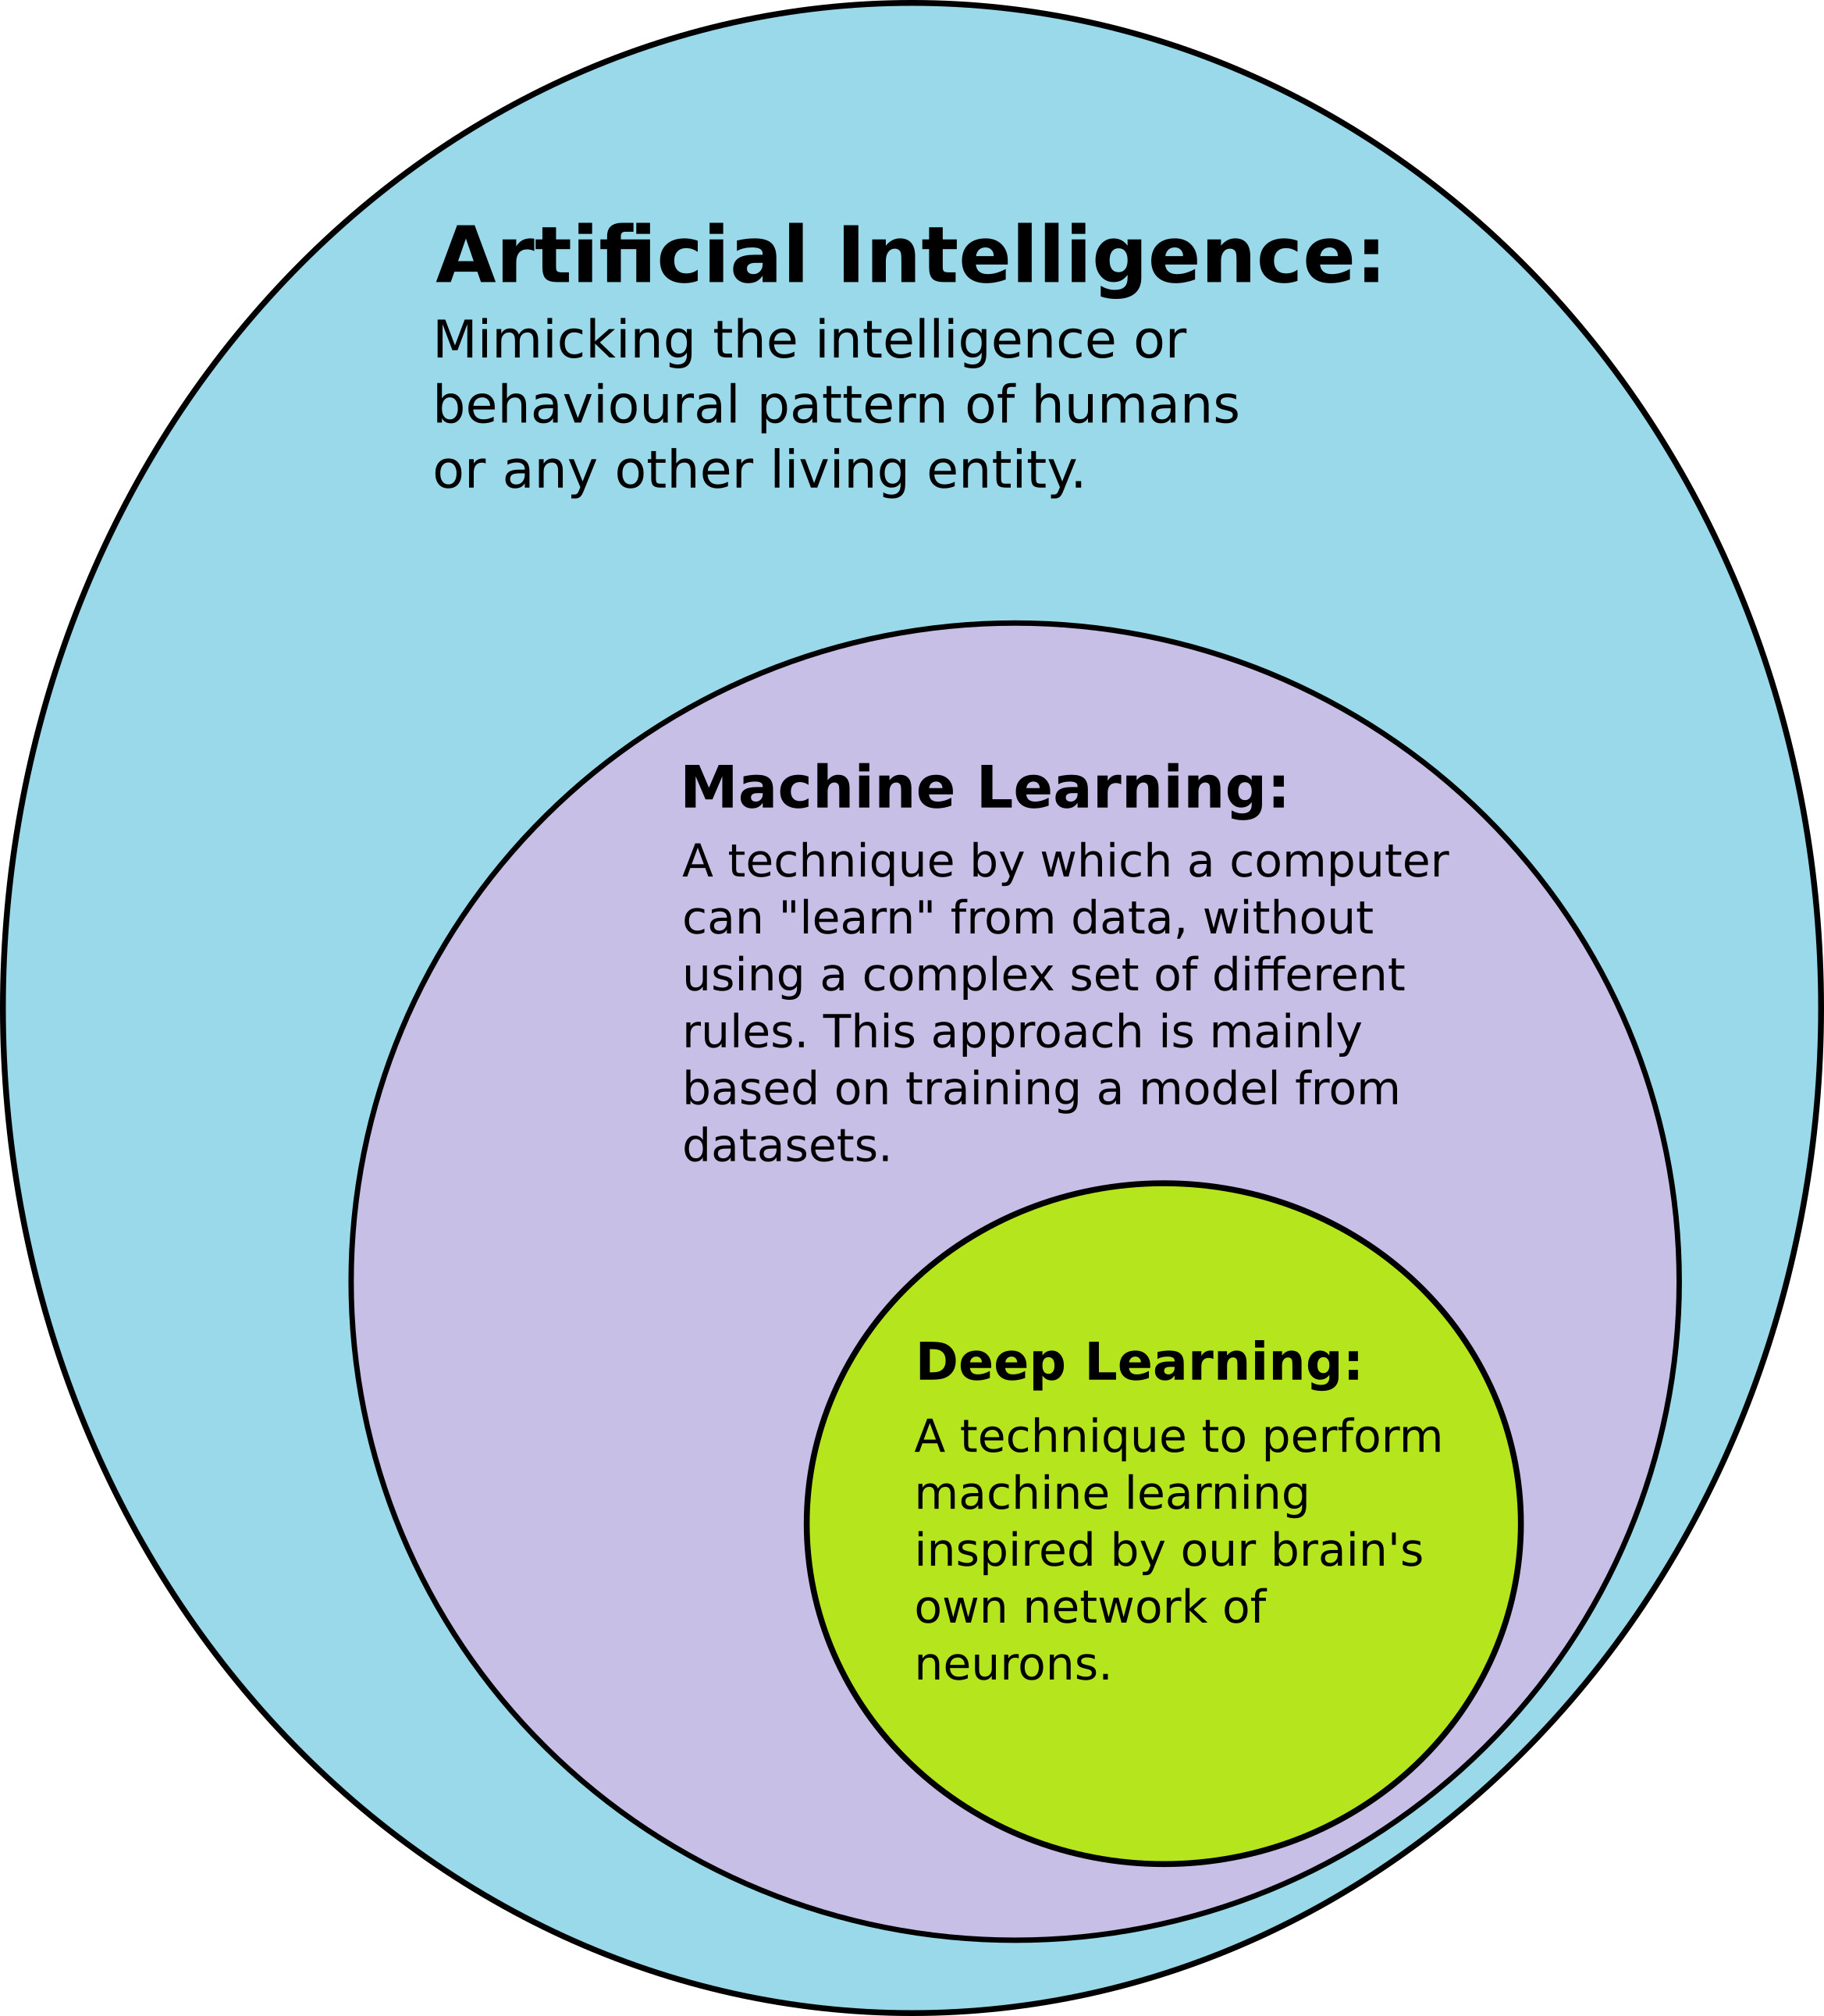
\includegraphics[width=0.5\textwidth]{images/chapter2/AI-ML-DL.jpg}
    \caption[Relazione tra IA, ML e DL.]{Relazione tra Intelligenza Artificiale, Machine Learning e Deep Learning. Tradotto: l'Intelligenza artificiale mima l'intelligenza od il comportamento di umani o qualsiasi altra entità vivente; il Machine Learning è una tecnica in cui il computer può "imparare" dai dati, senza utilizzare un insieme complesso di regole differenti. Questo approccio è principalmente basato sull'addestramento di un modello dai dati; il Deep Learning è una tecnica per eseguire un approccio di machine learning, ispirata dalla rete di neuroni del nostro del nostro cervello. Fonte: \url{https://en.wikipedia.org/wiki/Deep_learning}}
    \label{fig:ai_ml_dl}
\end{figure}

Una rete di base è costituita da uno strato di input, uno o più strati nascosti e uno strato di output di nodi interconnessi. Ogni nodo nascosto calcola una caratteristica che è una funzione dell'input ponderato che riceve dai nodi del livello precedente. Gli output vengono propagati a ogni livello successivo finché il livello di output non genera una classificazione \cite{ragoza_protein-ligand_2017}.

L'architettura della rete e la scelta della funzione di attivazione per ogni livello determinano il design della rete. I pesi che parametrizzano il modello sono in genere ottimizzati per adattarsi a un determinato set di dati di addestramento per ridurre al minimo l'errore della rete, senza eccedere nell'overfitting\footnote{In statistica e in informatica, si parla di overfitting o sovradattamento quando un modello statistico molto complesso si adatta ai dati osservati perché ha un numero eccessivo di parametri rispetto al numero di osservazioni. } \cite{ragoza_protein-ligand_2017}.

\section{CNN: Convolutional Neural Network}

Le \textit{reti neurali convoluzionali} (CNN) sono un tipo di rete neurale comunemente usata nel riconoscimento delle immagini. Le CNN scompongono gerarchicamente un'immagine in modo che ogni livello della rete impari a riconoscere le caratteristiche di livello superiore mantenendo le loro relazioni spaziali \cite{ragoza_protein-ligand_2017}.

Le applicazioni che richiedono il riconoscimento di oggetti e la visione artificiale, come i veicoli a guida autonoma e le applicazioni di riconoscimento facciale, si basano ampiamente sulle CNN.
Le impressionanti prestazioni delle CNN nell'attività di riconoscimento delle immagini suggeriscono che sono adatte per l'apprendimento da altri tipi di dati spaziali, come le strutture proteina-ligando \cite{ragoza_protein-ligand_2017}. 

\begin{figure}[H]
    \centering
    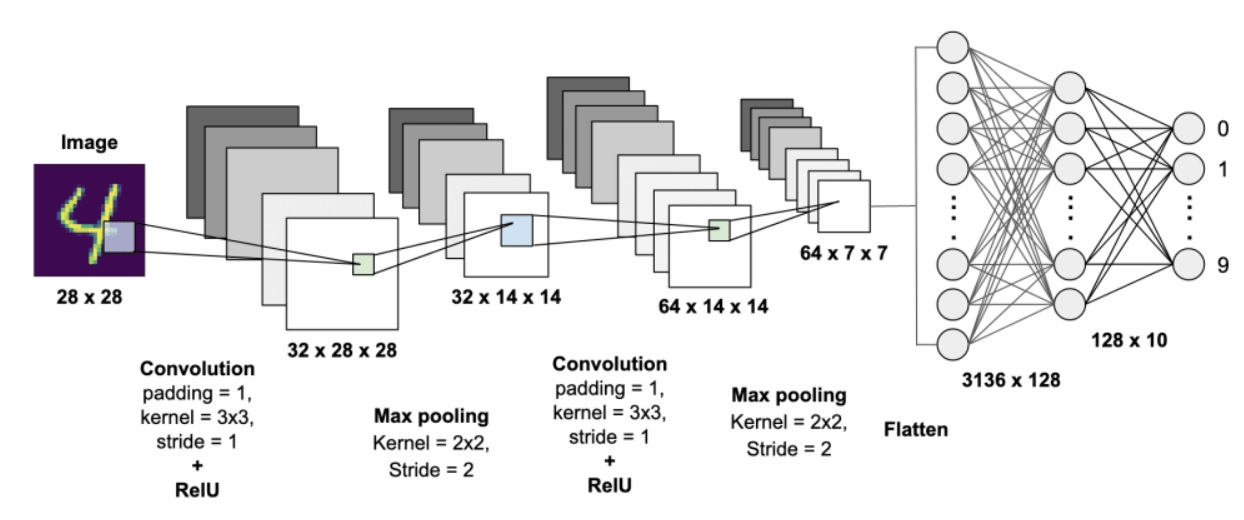
\includegraphics[scale=0.55]{images/chapter2/convNet.jpg}
    \caption[Esempio di CNN per il riconoscimento di numeri arabi.]{Esempio di rete neurale convoluzionale per il riconoscimento di numeri arabi. A sinistra l'immagine di input, al centro i layer del modello e la relativa funzione di attivazione, a destra la relativa rappresentazione come rete di neuroni. Fonte: \url{https://dev.to/afrozchakure/cnn-in-a-brief-27gg}}
    \label{fig:conv_net}
\end{figure}

L’utilizzo delle CNN per il deep learning è diffuso per via di tre fattori importanti:
\begin{itemize}
    \item eliminano la necessità di estrarre manualmente le \textbf{features} in quanto queste vengono apprese direttamente dalla CNN. Ciò consente l'estrazione di caratteristiche che non sono prontamente codificate in potenziali semplificati, come l'involucro idrofobico o termini dipendenti dalla superficie, così come le caratteristiche che non sono state ancora identificate come rilevanti da alcuna funzione di scoring esistente;
    \item producono risultati di riconoscimento ad alta precisione;
    \item possono essere addestrate nuovamente per nuove attività di riconoscimento, consentendo agli utenti di basarsi sulle reti preesistenti.
\end{itemize}

Le CNN rappresentano una tecnologia chiave in applicazioni come l'imaging biomedico, elaborazione audio, sistemi di guida autonoma e nella generazione di dati sintetici.

\subsection{Storia delle reti neurali convoluzionali}
Il primo modello teorico di un rudimentale neurone artificiale vede la luce nel 1943 grazie ad una coppia di scienziati, Warren Sturgis \textbf{McCulloch} (neurofisiologo) e Walter \textbf{Pitts} (matematico) nella loro pubblicazione \textit{“A logical calculus of the ideas immanent in nervous activity”}. 
I due descrivono un apparato in grado di ricevere \(n\) dati binari in ingresso in ognuno dei suoi elementi, a cui segue un singolo dato in uscita per ciascuno. Si dimostrò essere un "combinatore lineare a soglia", in grado di calcolare semplici funzioni booleane \cite{ai4b_reti_neurali, ia_reti_neurali}.

Nel 1949 lo psicologo canadese Donald Olding \textbf{Hebb} ipotizza la possibilità di istruire le macchine con un apprendimento che emuli quello alla base dell’intelligenza umana \cite{ia_reti_neurali}.

Nel 1958 viene proposta da Frank \textbf{Rosenblatt} (psicologo e computer scientist americano) la prima rete neurale: \textbf{Perceptron}, che possiede uno strato di nodi (neuroni artificiali) di input e un nodo di output.
I pesi sinaptici (un peso indica la forza di una connessione fra due nodi) sono dinamici, permettendo alla macchina di apprendere, in un modo sommariamente simile, anche se molto più elementare, a quello delle reti neurali biologiche. Il modello è feedforward: gli impulsi si propagano in un’unica direzione, in avanti. Tuttavia, il suo campo di applicazione è molto limitato \cite{ia_reti_neurali, ai4b_reti_neurali}.

Le teorie di Rosenblatt scaldano la comunità scientifica per oltre un decennio ma nel 1969 Marvin \textbf{Minsky} e Seymour \textbf{Papert} ne dimostrano i forti limiti: Perceptron risulta essere infatti una rete neurale poco potente, incapace di calcolare la funzione “or esclusivo” (XOR) \cite{ai4b_reti_neurali, camastra_machine_2015}.

Paul \textbf{Werbos}, nel 1974, descrive nella sua tesi di dottorato come impostare l’apprendimento di un MLP \cite{ia_reti_neurali}.

Nel 1986 David \textbf{Rumelhart} introduce il terzo strato delle reti neurali (hidden layers), che caratterizza il \textbf{Multi-Layer Perceptron} (MLP): al suo interno, fra i nodi di input e quello di output si trova uno strato hidden, dove avviene l’elaborazione delle informazioni provenienti dallo strato di input, che poi vengono inviate al nodo di output. È una rete feedforward non lineare: le connessioni in ingresso e in uscita da ogni singolo nodo sono multiple. A merito di tale architettura, il MLP può computare qualsiasi funzione. Inoltre, sempre nel 1986, David \textbf{Rumelhart}, Geoffrey \textbf{Hinton} (premio Turing) e Ronald \textbf{Williams} elaborano il celebre \textbf{Error Back-Propagation}, ancora oggi utilizzato, presentato nel libro \textit{"Parallel Distributed Processing"} \cite{ai4b_reti_neurali, ia_reti_neurali, camastra_machine_2015}.

L’EBP permette di perfezionare in stadi successivi l’apprendimento automatico di una rete neurale. Si implementa modificando i pesi delle connessioni fra nodi che non producono l’output ottimale, finché non si ottiene quest’ultimo \cite{ia_reti_neurali}.

Dalla fine degli anni ’80, con l’arrivo sul mercato di nuovi potenti processori e avanzati chip in grado di supportare applicazioni intensive come quelle delle analisi e delle simulazioni, il percorso di avanzamento tecnologico dell’hardware non si è più arrestato \cite{ai4b_reti_neurali}. 

Allo stato attuale dell'arte, nei laboratori di ricerca si sta lavorando ai \textbf{chip neuromorfici} (che imitano il funzionamento del cervello umano) e a quelli per il \textbf{quantum computing} \cite{ai4b_reti_neurali}{}.

\subsection{Apprendimento delle feature, layer e classificazione} \label{cnn}
Analogamente ad altre reti neurali, una CNN è costituita da un layer di input, un layer di output e tanti layer intermedi nascosti.

\begin{figure}[H]
    \centering
    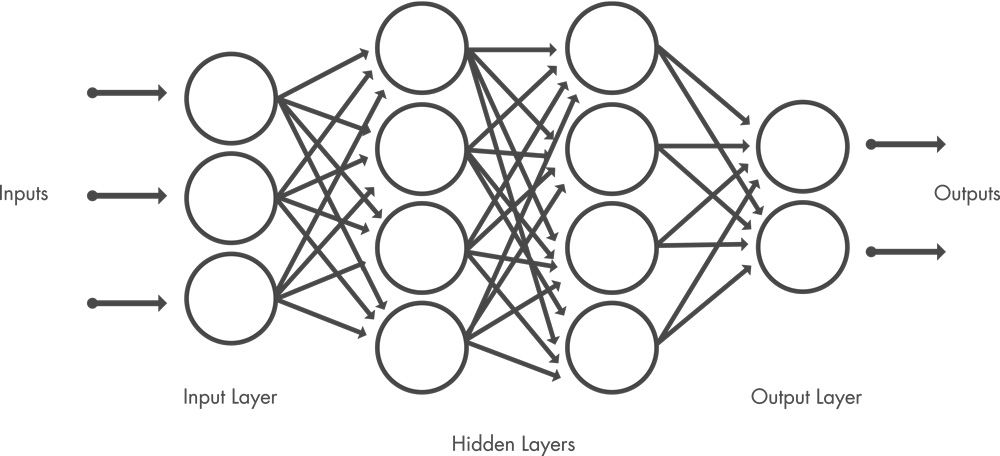
\includegraphics[scale=0.34]{images/chapter2/cnn_layers.jpg}
    \caption[Esempio di rete neurale per il deep learning.]{Esempio di rete neurale \textit{fully connected} per il deep learning. La figura mostra lo strato di input, gli strati intermedi nascosti e lo strato di output. Fonte: \url{https://it.mathworks.com/discovery/convolutional-neural-network-matlab.html}}
    \label{fig:cnn_layers}
\end{figure}

Questi layer eseguono operazioni che alterano i dati al fine di apprendere le feature specifiche dei dati stessi. Tre dei layer più diffusi sono: la convoluzione, l’attivazione o ReLU e il pooling.

La \textbf{convoluzione} sottopone le immagini di input a una serie di filtri convoluzionali, ciascuno dei quali attiva determinate feature dalle immagini.

Nella definizione di un layer convoluzionale vengono considerati:
\begin{itemize}
    \item \textbf{kernel size}: rappresenta le dimensioni della matrice del kernel di convoluzione;
    \item \textbf{padding}: rappresenta le dimensioni del bordo esterno applicato alla immagine di input;
    \item \textbf{stride}: rappresenta la velocità di traslazione del kernel sull’immagine, misurata in pixel orizzontali e verticali;
    \item \textbf{numero di filtri}: un layer convoluzionale gestisce un certo numero di kernel in contemporanea che vengono applicati alla stessa immagine in input, in modo da ottenere subito tanti filtri diversi.
\end{itemize}

La \textbf{Rectified Linear Unit} (ReLU), in italiano unità lineare rettificata, consente di eseguire un addestramento più rapido ed efficace mappando i valori negativi a zero e mantenendo quelli positivi. Questa operazione è talvolta definita attivazione, dal momento che solo le feature attivate vengono trasmesse al layer successivo.

Il \textbf{pooling} semplifica l’output mediante l’esecuzione di un sottocampionamento non lineare, riducendo in tal modo il numero di parametri che la rete deve apprendere.
Queste operazioni vengono reiterate su decine o centinaia di layer e ciascun layer impara ad identificare feature diverse \cite{mathworks_cnn}.
Attraverso il \textit{max pooling}, si mantiene il valore massimo per ciascuna convoluzione mentre con l'\textit{average pooling}, si considera il valore medio.

\subsection{Gestione di pesi e bias}
Analogamente a una rete neurale tradizionale, una CNN possiede \textbf{neuroni con pesi} e \textbf{bias}. Il modello apprende questi valori durante l’addestramento e li aggiorna costantemente con ogni nuovo esempio di addestramento. Tuttavia, nel caso delle CNN, i valori dei pesi e dei bias sono gli stessi per tutti i neuroni nascosti in un determinato layer.

Ciò significa che tutti i neuroni nascosti rilevano la stessa feature, come bordi o macchie, in diverse aree dell’immagine. Ciò rende la rete tollerante alla traslazione di oggetti in un’immagine. Ad esempio, una rete addestrata a riconoscere automobili sarà in grado di farlo indipendentemente dal tipo di automobile presente nell’immagine \cite{mathworks_cnn}.

\subsection{Layer di classificazione}
Dopo aver appreso le feature in numerosi layer, l’architettura di una CNN passa alla \textbf{classificazione}.

Il penultimo layer è un layer completamente connesso che emette un vettore di dimensioni \(K\) dove \(K\) è il numero di classi che la rete sarà in grado di prevedere. Questo vettore contiene le probabilità per ciascuna classe di qualsiasi immagine classificata.

L’ultimo layer dell’architettura CNN utilizza un layer di classificazione come una \textbf{softmax} per fornire l’output della classificazione \cite{mathworks_cnn}, che trasforma l'input dell'output layer della rete neurale in un vettore delle probabilità, la cui somma è pari ad 1.


\section{GNINA}
% Gnina 
GNINA è un fork di \textit{smina}\footnote{\textit{smina} è un software di docking computazionale, costruito sulla base di AutoDock Vina, in grado di supportare funzioni di scoring personalizzate e la minimizzazione di energia ad alte prestazioni \cite{koes_lessons_2013}.}, che a sua volta è un fork di Vina, è un programma di docking molecolare con supporto integrato per il calcolo del punteggio e l'ottimizzazione della posa dei ligandi utilizzando reti neurali convoluzionali, sotto licenza GPL e Apache \cite{mcnutt_gnina_2021}. 

L'utilizzo di modelli CNN richiede una notevole potenza di calcolo, fornita dalle moderne schede grafiche (GPU), per ottenere risultati in tempi modesti. Per tal motivo, GNINA fa riferimento a molte più dipendenze tra cui CUDA\footnote{CUDA (acronimo di Compute Unified Device Architecture) è un'architettura hardware per l'elaborazione parallela creata da NVIDIA. Tramite l'ambiente di sviluppo per CUDA, i programmatori di software possono scrivere applicazioni capaci di eseguire calcolo parallelo sulle GPU delle schede video NVIDIA.} \cite{mcnutt_gnina_2021}.

GNINA consente all'utente di utilizzare i modelli CNN come funzioni di scoring all'interno della pipeline di docking in vari modi. Le varie opzioni di punteggio CNN consentono ai modelli CNN specificati di sostituire la funzione di scoring nelle fasi di "sampling", "refinement" e "rescoring" \cite{mcnutt_gnina_2021}. 


\subsection{Funzionamento della pipeline di GNINA}
Come illustra la Figura \ref{fig:gnina_pipeline}, GNINA prevede una pipeline di docking ben specifica, in parte implementata anche in altri software di docking computazionale. In particolare, la fase di campionamento è stata ampiamente descritta nella Sezione \ref{implementazione_docking};  per valutare il punteggio per la conformazione minimizzata, è utilizzato il criterio di Metropolis.

Ciascuna catena di Monte Carlo conserva le conformazioni del ligando con il punteggio più alto ed, a seguito del campionamento, le conformazioni salvate da ciascuna catena vengono aggregate; le conformazioni dal punteggio più alto vengono conservate per ulteriori analisi \cite{mcnutt_gnina_2021}. 

\vspace{0.5cm}
\begin{figure}[H]
    \centering
    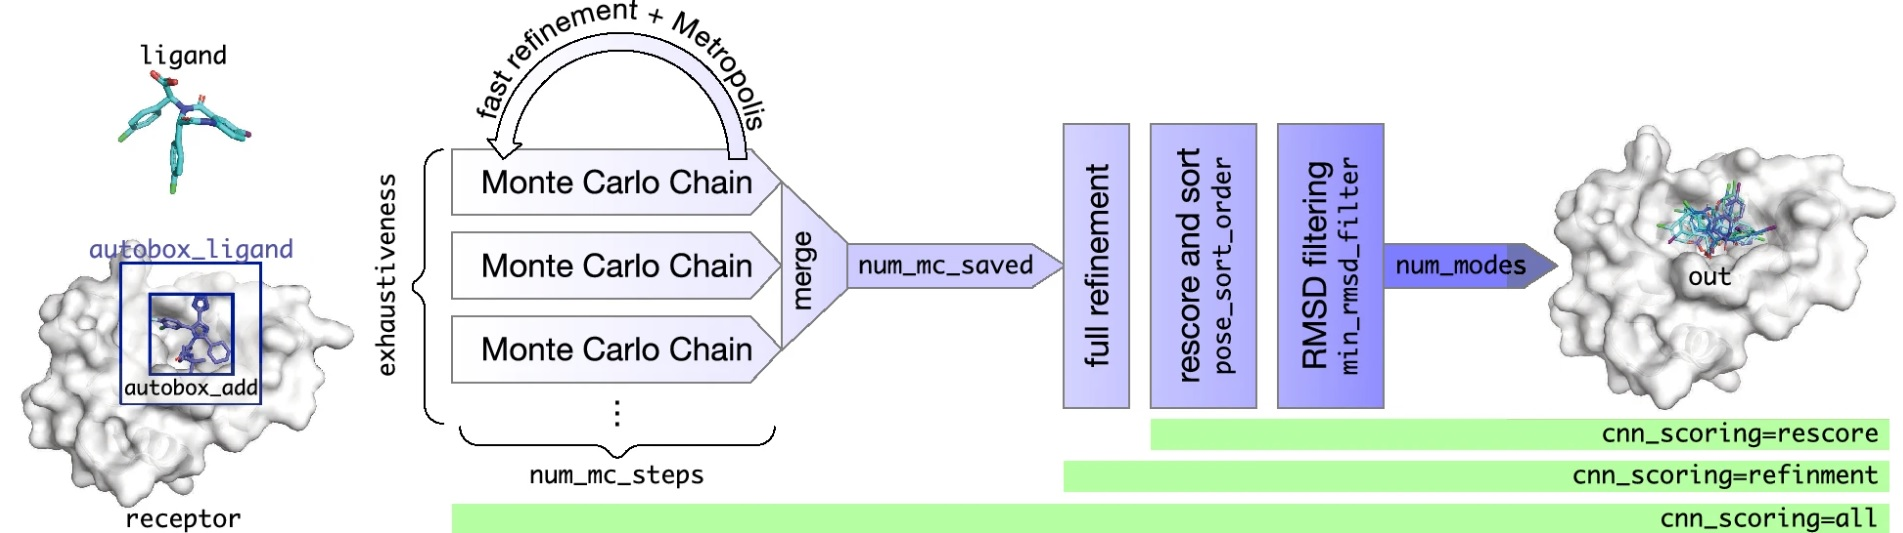
\includegraphics[scale=0.35]{images/chapter2/gnina_pipeline.jpg}
    \caption[Pipeline di docking seguita da GNINA.]{Pipeline di docking seguita da GNINA. A sinistra, viene mostrata la differenza tra autobox_add ed autobox_ligand. A seguito, vengono mostrate le fasi del processo di docking, fornendo indicazioni sui parametri coinvolti, modificabili dall'utente. Fonte: \cite{mcnutt_gnina_2021}}
    \label{fig:gnina_pipeline}
\end{figure}

Le conformazioni con il punteggio più alto vengono quindi perfezionate applicando nuovamente una funzione di scoring, empirica o CNN, al fine di ottenere la posa localmente ottimale.
Il perfezionamento sposta la posa del ligando a un minimo di energia locale utilizzando i gradienti della funzione di scoring. Dopo che la posa del ligando è stata perfezionata, le affinità finali e i punteggi vengono calcolati per la posa utilizzando i modelli CNN specificati e/o la funzione di punteggio specificata. Infine, le conformazioni del punteggio più alto sono ordinate ed esportate con Open Babel \cite{mcnutt_gnina_2021}. 

\subsection{Modelli CNN in GNINA}
Dopo aver introdotto nella Sezione \ref{cnn} la struttura di una rete neurale convoluzionale ed i layers più comuni, è possibile farsi un'idea più chiara del modello utilizzato da GNINA per valutare le pose. 

\begin{figure}[H]
    \centering
    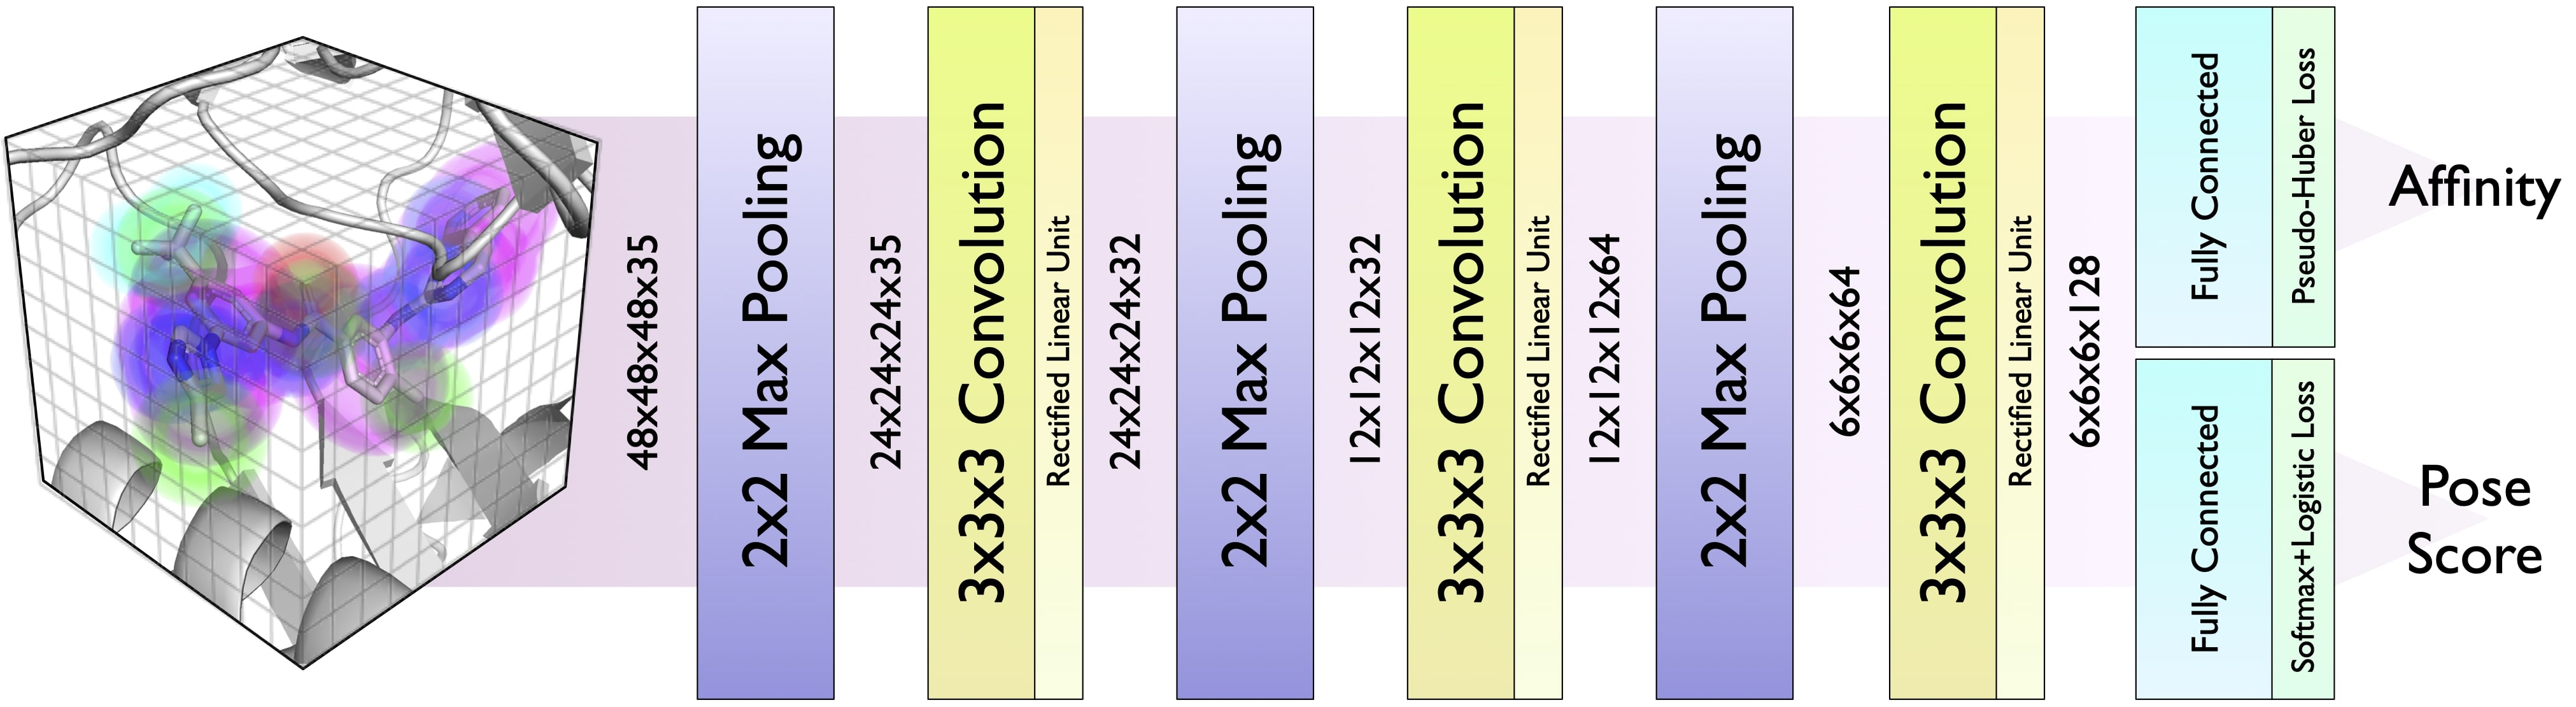
\includegraphics[scale=0.09]{images/chapter2/cnn_model.jpg}
    \caption[Modello CNN predefinito utilizzato da GNINA.]{Modello CNN predefinito utilizzato da GNINA. In generale le reti convoluzionali sono formate da una sequenza di layer convoluzionali e di pooling, seguita da una rete di classificazione. Fonte: \cite{mcnutt_gnina_2021}}
    \label{fig:cnn_model}
\end{figure}

La funzione di scoring CNN predefinita è un insieme di 5 modelli selezionati per bilanciare le prestazioni di previsione della posa e il tempo di esecuzione: dense, general\_default2018\_3, dense\_3, crossdock\_default2018 e redock\_default2018 \cite{mcnutt_gnina_2021}.


Le funzioni di scoring CNN possono essere specificate fornendo dei file di modello e/o di pesi oppure selezionando un modello built-in. 
I modelli CNN built-in disponibili riguardano crossdock\_ default2018, dense, general\_default2018, redock\_default2018, e default2017, ognuno di questi è addestrato utilizzando un diverso dataset di training e/o un'architettura di modello differente. Inoltre, ogni modello, eccetto per default2017, ha cinque varianti che sono addestrate sugli stessi dati e hanno la stessa architettura, ma sono inizializzati con un seme casuale diverso \cite{mcnutt_gnina_2021}. 


Per ogni tipo di modello CNN, il nome del modello di base si riferisce alla variante con le prestazioni di docking più elevate, e le restanti varianti sono numerate sequenzialmente (ad esempio general\_default2018, general\_ default2018\_1, general\_default2018\_2, general\_default2018\_3, e general\_ default2018\_4); l'insieme di queste cinque varianti è denotato con '\_ensemble' (ad esempio general\_default2018\_ensemble) \cite{mcnutt_gnina_2021}. 

I calcoli ad alte prestazioni della CNN sono eseguiti utilizzando cuDNN, un framework di deep learning  ottimizzato per le GPU, incluso in Caffe. Questi modelli sono addestrati per predire sia la qualità della posa (una probabilità che la posa abbia un RMSD basso rispetto alla posa di legame) e l'affinità di legame (pK). 
Il punteggio della posa è utilizzato per tutti i processi di ottimizzazione della posa \cite{mcnutt_gnina_2021}.

Di seguito sono riportati alcuni dei modelli finalizzati a scopi differenti, come la qualità della posa per HiRes Pose oppure la predizione di affinità migliore come HiRes Affinity.
\begin{figure}[H]
    \centering
    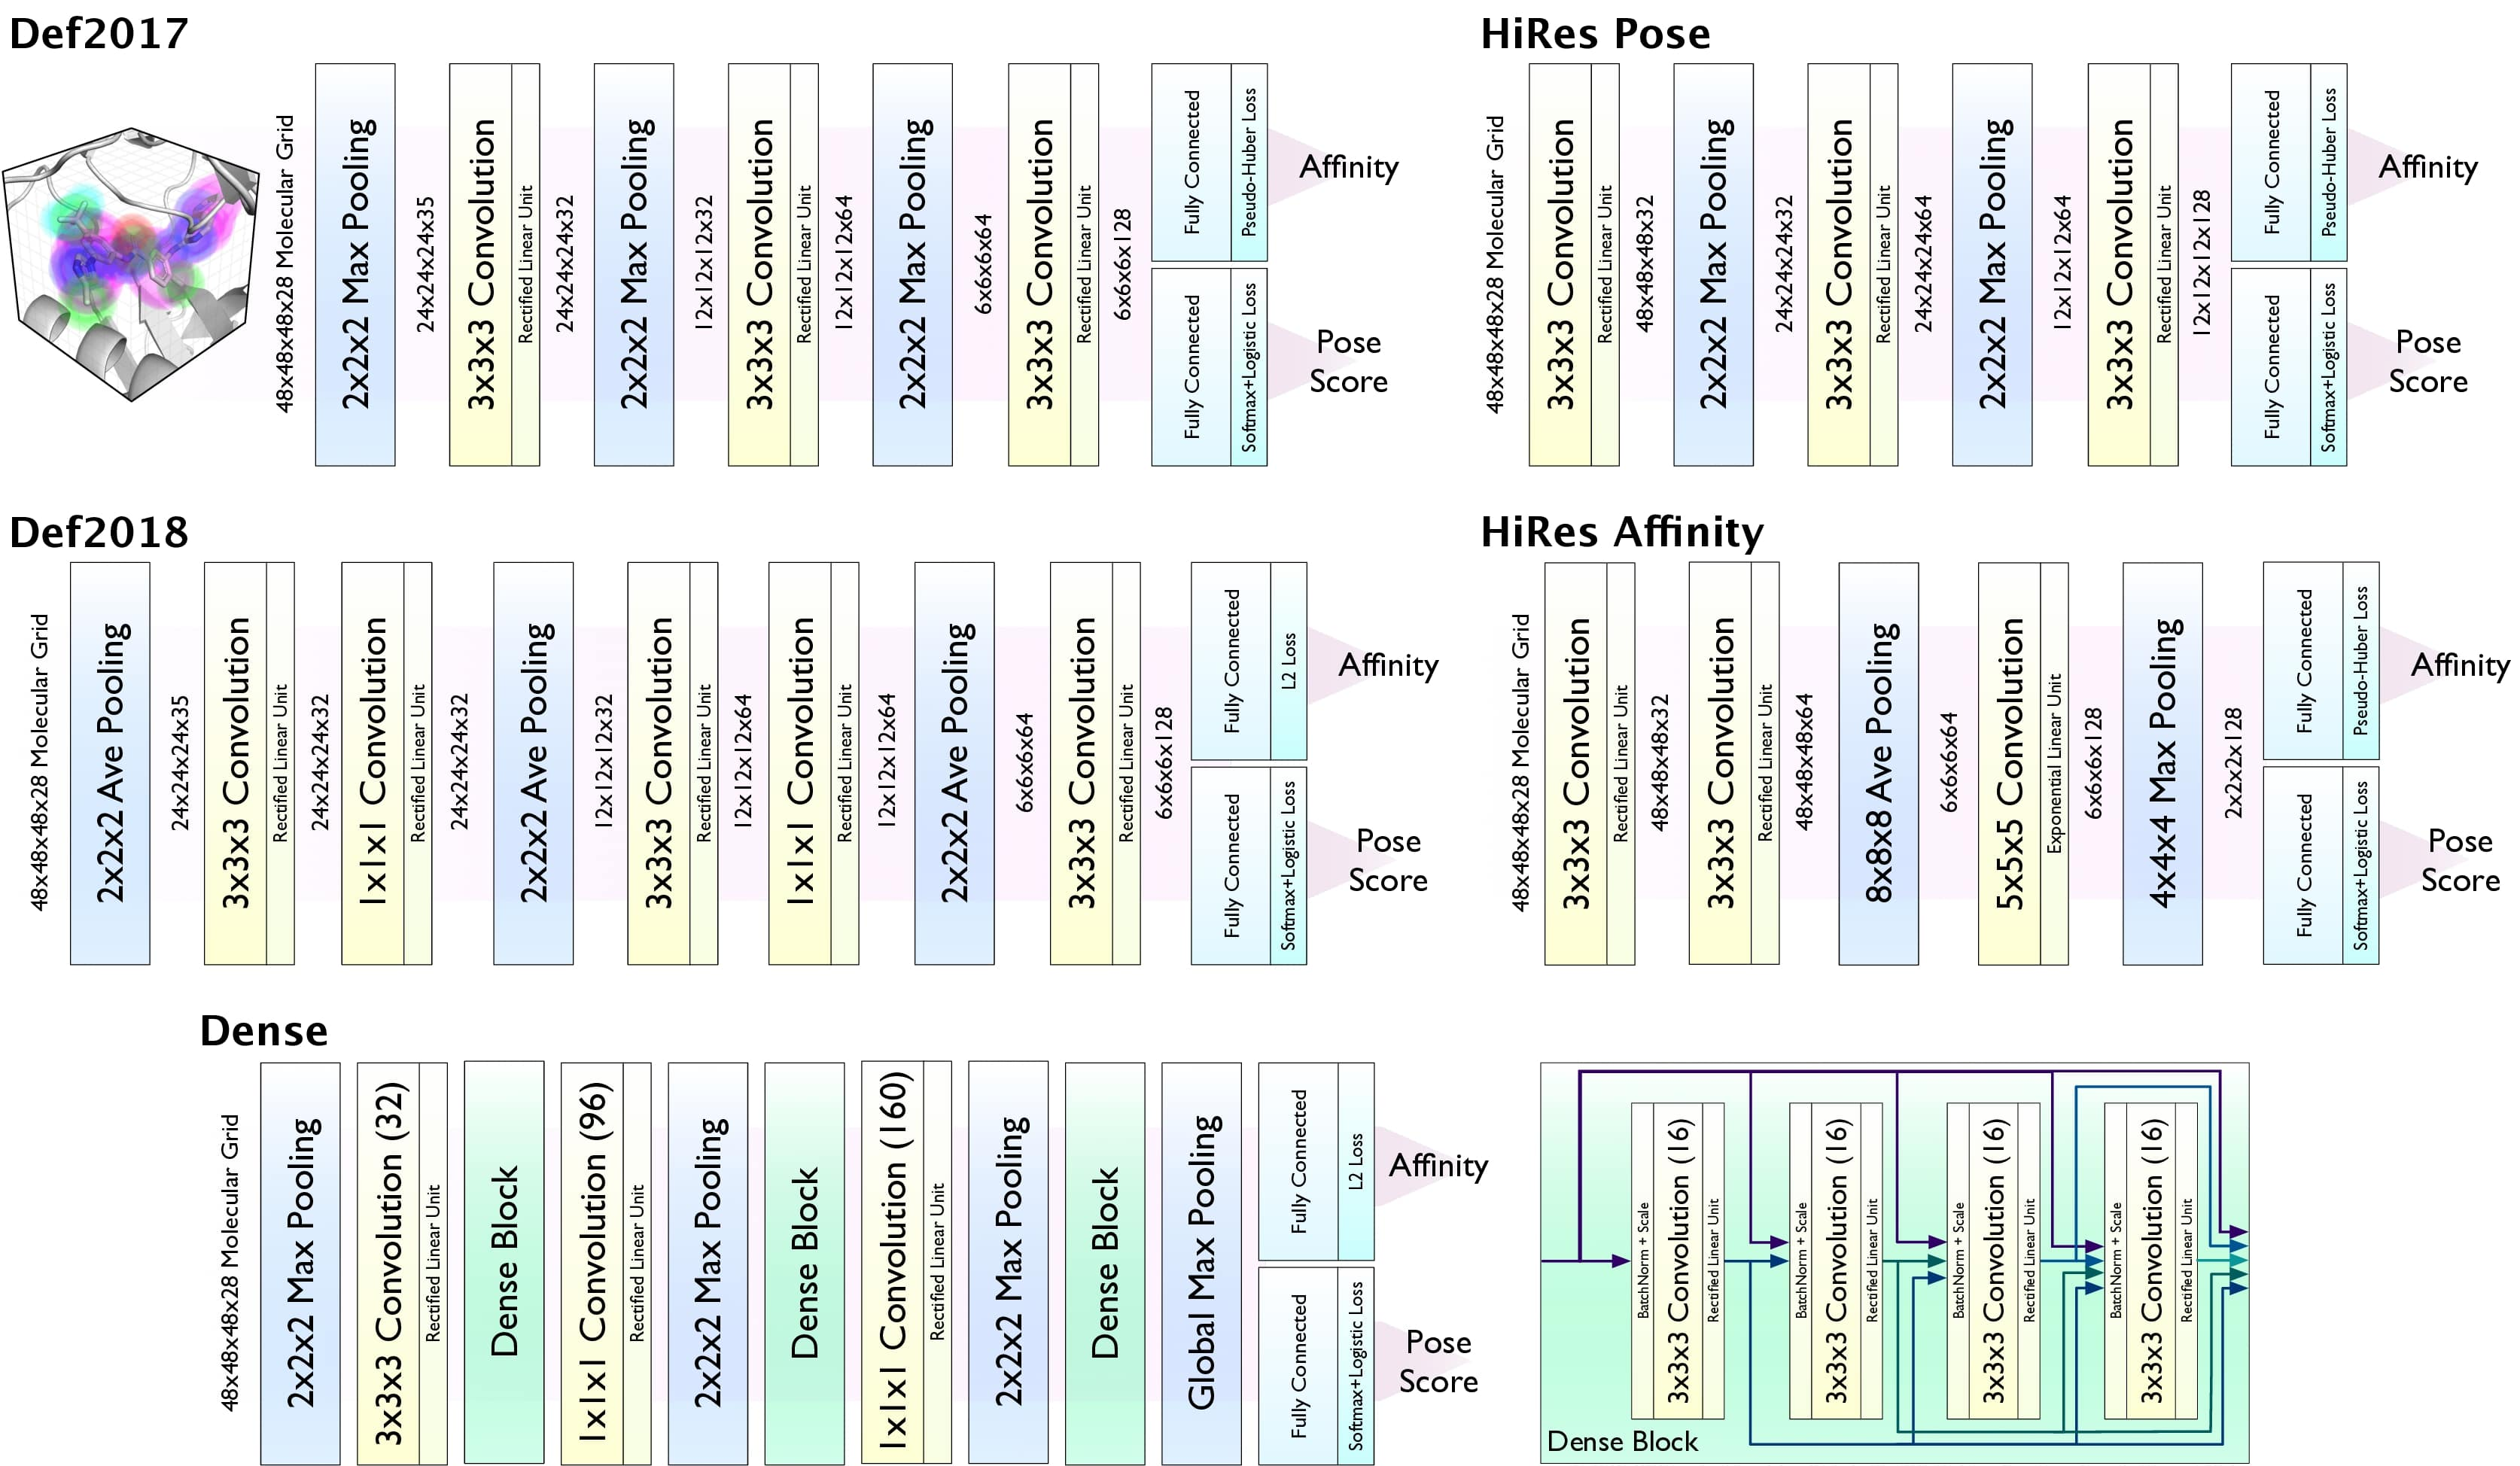
\includegraphics[scale=0.12]{images/chapter2/models.jpg}
    \caption[Esempi di modelli CNN built-in di GNINA.]{Esempi di modelli CNN built-in di GNINA. I modelli sono etichettati con i loro nome ed per ciascun modello è riportata la propria struttura. Fonte: \cite{mcnutt_gnina_2021}}
    \label{fig:models}
\end{figure}

\subsection{Parametri della CNN in GNINA} \label{cnn_params}
I parametri messi a disposizione per l'utilizzo della CNN nel docking molecolare sono molteplici. Tuttavia, ci focalizziamo sui parametri interessanti ed utilizzati per l'analisi sperimentale proposta dall'elaborato.

Un modello CNN prevede sia la qualità della posa (CNNScore) che l'affinità di legame (CNNaffinity) per ciascuna delle conformazioni prodotte da GNINA. 

Il parametro \textbf{CNNscore} è una stima della bontà della posa ed è un valore compreso tra 0 e 1 che viene utilizzato per classificare le pose del ligando. Un valore di CNNscore pari ad 1 denota una posa del ligando perfetta (rispetto al ligando naturale ove presente). Tendenzialmente, le pose di ligandi molto vicine al recettore, ovvero entro un valore di RMSD inferiore a 2, risultano essere qualitativamente migliori secondo questo criterio \cite{mcnutt_gnina_2021}.

Il parametro \textbf{CNNaffinity} è l'affinità prevista dopo aver stabilito una posa valida nel processo di docking, in questo caso come determinato dalla CNN. E' misurata in unità \(pK\)\footnote{Il valore \(pK\) è un metodo utilizzato per indicare la forza di un composto, relativamente alla costante di dissociazione \(K\).
Un valore di \(pK\) basso indica un composto forte.} \cite{mcnutt_gnina_2021}.

Il parametro \textbf{autobox\_ligand} è ereditato da \textit{smina} e consente di creare una box che inscrive esattamente le coordinate dell'atomo del ligando fornito ed in seguito espansa con il parametro autobox\_add (predefinito 4Å) in ogni dimensione \cite{mcnutt_gnina_2021}.

Il parametro \textit{cnn\_scoring} determina in quali punti della procedura di docking viene utilizzata la funzione di scoring CNN:
\begin{itemize}
    \item \textbf{none} (nessuno) - nessuna CNN utilizzata per il docking. Utilizza la funzione di scoring Vina durante l'intero processo;
    \item \textbf{rescore (predefinito)} - la CNN è utilizzata per riclassificare le pose finali. Risulta essere l'opzione meno costosa dal punto di vista computazionale, tra quelle che coinvolgono la CNN;
    \item \textbf{refinement} (perfezionamento) - la CNN è utilizzata per perfezionare le pose dopo le catene Monte Carlo e per il ranking finale delle pose di output. Risulta essere 10 volte più lento dell'opzione \textit{rescore} quando si utilizza una GPU;
    \item \textbf{all} (tutto) - la CNN è utilizzata come funzione di scoring durante l'intero processo. Questo risulta essere estremamente intensivo dal punto di vista computazionale e non consigliato \cite{mcnutt_gnina_2021}.
\end{itemize}
Le opzioni elencate ed illustrate nella Figura \ref{fig:cnn_scoring} per il parametro \textit{cnn\_scoring} verranno esplicate dettagliatamente nella Sezione \ref{cnn_scoring_method}.

Le pose risultanti vengono rivalutate e ordinate attraverso la selezione del parametro \textbf{pose\_sort\_order}:
\begin{itemize}
    \item \textbf{CNNscore (predefinito)} - le pose con la più alta probabilità di avere un RMSD basso secondo la CNN sono classificate più alte;
    \item \textbf{CNNaffinity} - le pose con la più alta affinità di legame prevista dalla CNN sono classificate più alte;
    \item \textbf{Energy} - le pose con l'energia più bassa o affinità predetta dalla funzione di scoring Vina sono classificate più alte;
\end{itemize}

Si nota che la modifica del criterio di ordinamento può modificare le pose restituite, non solo il loro ordinamento.

\subsection{Funzione di scoring CNN} \label{cnn_scoring_method}
GNINA consente l'utilizzo della CNN in varie fasi del processo di docking molecolare. 
Se la CNN non viene utilizzata affatto nel calcolo del punteggio (opzione \textit{"none"}), la pipeline di docking molecolare è essenzialmente la stessa di \textit{smina}. 
L'opzione \textit{rescore} ha il costo computazionale più basso delle opzioni che utilizzano i modelli CNN.
Con questa opzione i modelli CNN vengono utilizzati per valutare e riordinare le conformazioni del ligando selezionate e perfezionate dalla funzione di scoring non-CNN, la funzione di scoring predefinita Vina \cite{mcnutt_gnina_2021}. 

Per un costo computazionale aggiuntivo, è possibile specificare l'opzione "refinement" per utilizzare i modelli CNN per il perfezionamento dei ligandi dopo che sono stati selezionati dalle catene Monte Carlo. 
Oltre a perfezionare le conformazioni del ligando, i modelli CNN vengono utilizzati per valutare e riordinare le pose di output, come fa l'opzione "rescore". Tuttavia, le catene Monte Carlo continuano a utilizzare la funzione di scoring non-CNN \cite{mcnutt_gnina_2021}. 

\begin{figure}[H]
    \centering
    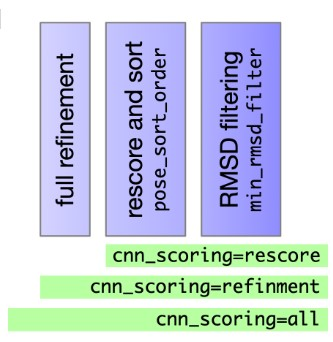
\includegraphics{images/chapter2/cnn_scoring.jpg}
    \caption[Fasi ricoperte dalle opzioni per il parametro cnn\_scoring.]{Illustrazione grafica delle fasi ricoperte per ciascun opzione del parametro cnn\_scoring. L'opzione \textit{all} applica il modello CNN all'intera pipeline; l'opzione \textit{refinement} è applicata alle fasi mostrate; l'opzione \textit{rescore} applica il modello CNN solo alle ultime due fasi prima di fornire l'output. Fonte: \cite{mcnutt_gnina_2021}}
    \label{fig:cnn_scoring}
\end{figure}

Il processo di \textit{refinement} o perfezionamento con i modelli CNN non è raccomandato in quanto il costo di calcolo è significativo e le prestazioni sono inferiori rispetto al semplice utilizzo dei modelli CNN per rivalutare le pose perfezionate dalla funzione di scoring Vina \cite{mcnutt_gnina_2021}.

L'opzione \textit{all} utilizza i modelli CNN come funzione di scoring nel corso della procedura di docking molecolare ed ha il costo computazionale più alto per ordini di grandezza. Il modello CNN viene utilizzato per il processo di selezione all'interno delle catene Monte Carlo, il processo di \textit{refinement} dopo la selezione Monte Carlo e nel calcolo del punteggio e del riordinamento delle pose prima dell'output. 
Questa opzione è molto impegnativa dal punto di vista computazionale poiché la CNN viene regolarmente interrogata per l'energia di una particolare conformazione durante la procedura di campionamento Monte Carlo \cite{mcnutt_gnina_2021}. 

GNINA consente di combinare le funzioni di scoring CNN e non-CNN, attraverso l'utilizzo di alcuni parametri, sia nella fase di perfezionamento che nel calcolo del punteggio di una certa posa.
L'utilizzo classico delle CNN all'interno della pipeline di docking di GNINA richiede un'elevata precisione limitando, al tempo stesso, i costi computazionali \cite{mcnutt_gnina_2021}.


\subsection{Formato dei dati di input e di output in GNINA}
Le strutture del recettore e del ligando possono essere fornite in qualsiasi formato, grazie alla facile gestione attraverso OpenBabel. Questa è una delle funzionalità ereditate da \textit{smina}. 

I parametri di output come CNNscore, CNNaffinity, così come la struttura stessa della posa finale, sono memorizzati nel file di output. Tendenzialmente, se si è interessati ai parametri allora il formato di output preferito dovrebbe essere il formato SDF.


\section{AutoDock Vina} 
Il software AutoDock Vina, progettato e realizzato dal Dr. Oleg Trott presso lo Scripps Research Institute e pubblicato nel 2009 sotto licenza Apache open source, è stato sviluppato per soddisfare l'esigenza di un metodo di docking che non richieda una conoscenza approfondita da parte degli utenti. È altamente ottimizzato per eseguire esperimenti di docking utilizzando metodi predefiniti ben testati  \cite{forli_computational_2016, eberhardt_autodock_nodate}. 

E' stato progettato per essere uno strumento di docking computazionale generico, che accetta file di coordinate per recettore e ligando ed effettua predizioni sulle conformazioni proteina-ligando ottimali \cite{forli_computational_2016}.
AutoDock Vina rappresenta un punto di riferimento per il docking computazionale e per tutte le sue applicazioni.

\subsection{Funzione di scoring Vina} \label{scoring_function_vina}
In Autodock Vina, per determinare quale ligando ha un'interazione complessa stabile con la proteina, la posa viene valutata in termini di "binding energy" o più comunemente affinità.
La funzione di scoring Vina è stata progettata per risultare un ottimo compromesso tra previsione della posa e dell'affinità e tempo di esecuzione ed è una somma pesata di interazioni atomiche \cite{koes_lessons_2013}. 

Ciascuno di questi termini rappresenta generalmente un importante fattore energetico nel legame proteina-ligando. 
Ci sono diversi parametri coinvolti in ciascuna di queste funzioni che possono essere modificati per migliorare le previsioni. Infine, ogni termine viene pesato (moltiplicato per una costante) prima di essere aggiunto all'affinità di legame finale prevista \cite{quiroga_vinardo_2016}. 

L'energia di legame è prevista come la somma delle interazioni di coppie di atomi dipendenti dalla distanza \ref{eq:1}.

\begin{equation} \label{eq:1}
    E = \sum{e_{pair}}{(d)}
\end{equation} 

Qui \(d\) è la distanza superficiale calcolata con l'Equazione \ref{eq:2}, dove r è la distanza interatomica e \(R_i\) e \(R_j\) sono i raggi degli atomi nella coppia \cite{quiroga_vinardo_2016}. 

\begin{equation} \label{eq:2}
    d = r - R_i - R_j
\end{equation} 

Ogni coppia di atomi interagisce attraverso un'interazione sterica data dai primi tre termini dell'Equazione \ref{eq:3}. 
Inoltre, a seconda del tipo di atomo, potrebbero esserci interazioni idrofobiche e non direzionali di legame a idrogeno, date dagli ultimi due termini dell'Eq \ref{eq:3} \cite{quiroga_vinardo_2016}.

\begin{equation} \label{eq:3}
    e_{pair}(d) = 
    \begin{cases}
        w_1 * \text{Gauss}_1(d) +\\
        w_2 * \text{Gauss}_2(d) +\\
        w_3 * \text{Repulsion}(d) +\\
        w_4 * \text{Hydrophobic}(d) +\\
        w_5 * \text{HBond}(d)
    \end{cases}
\end{equation} 

I pesi dei termini sono stati calcolati tramite un adattamento non lineare ai dati strutturali. La Tabella \ref{vina_weights} riporta i termini ed i pesi riferiti nell'Equazione \ref{eq:3} \cite{quiroga_vinardo_2016}.

\begin{table}[H] 
\centering
\begin{tabular}{|l|c|}
\hline
\rowcolor[HTML]{C0C0C0} 
\multicolumn{1}{|c|}{\cellcolor[HTML]{C0C0C0}\textbf{Termine}} & \textbf{Peso} \\ \hline
Gauss\_1                                                       & -0-0356       \\ \hline
Gauss\_2                                                       & -0.00516      \\ \hline
Repulsion                                                      & 0.840         \\ \hline
Hydrophobic                                                    & -0-0351       \\ \hline
Hydrogen bonding                                               & -0.587        \\ \hline
\end{tabular}
\caption[Termini e pesi della funzione di scoring Vina.]{Termini e pesi della funzione di scoring Vina. I termini sono direttamente codificati nel codice sorgente di AutoDock Vina. Fonte: \cite{trott_autodock_2009}}
\label{vina_weights}
\end{table}

È stato dimostrato che si comporta bene con ligandi con dimensioni e composizione biologiche tipiche in esperimenti di \textit{blind docking}.
Per una descrizione più dettagliata della funzione di scoring Vina, si rimanda il lettore all'articolo originale di Trott e Olson \cite{trott_autodock_2009, quiroga_vinardo_2016}.

Nell'implementazione della funzione di scoring Vina, viene utilizzato il metodo di ottimizzazione non lineare non vincolata \textbf{Broyden-Fletcher-Goldfarb-Shanno}, già descritto nella Sezione \ref{bfgs}.

\subsection{Formato dei dati di input ed ouput in AutoDock Vina}
Il successo del docking computazionale e dello screening virtuale richiede un'attenta attenzione alla qualità delle coordinate utilizzate per recettori e ligandi. AutoDock Vina utilizza una rappresentazione semplificata delle molecole, memorizzata nel formato PDBQT, un'estensione del formato PDB \cite{forli_computational_2016}.

Ciò semplifica l'utilizzo di Vina con il software ausiliario esistente sviluppato per AutoDock, come AutoDock Tools, per la preparazione dei file, la scelta dello spazio di ricerca e la visualizzazione dei risultati. \cite{trott_autodock_2009}

Il formato PDBQT è un formato più ricco di espressività rispetto al formato standard PDB in quanto, permette di modellare la struttura molecolare come una struttura ad albero.

\begin{figure}[H]
    \centering
    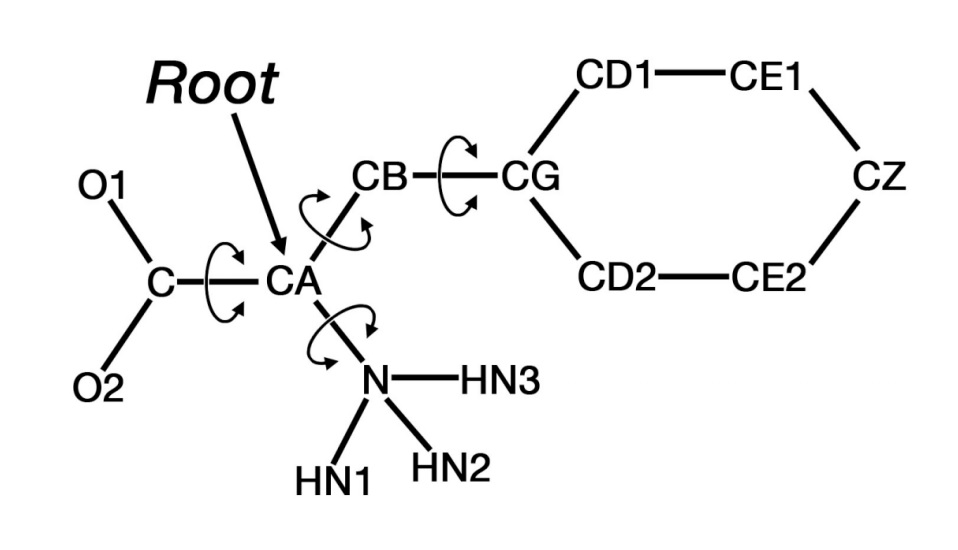
\includegraphics[scale=0.5]{images/chapter2/pdbqt.jpg}
    \caption[Rappresentazione grafica del formato PDQBT.]{Rappresentazione grafica della struttura ad albero codificata all'interno del formato PDQBT. Fonte: \cite{eberhardt_autodock_nodate}}
    \label{fig:pdbqt}
\end{figure}

\section{Linguaggi di programmazione}
\subsection{Python}
L'applicazione è scritta prevalentemente in \textbf{Python3}, anche se alcuni script fanno riferimento a Python2. La scelta di tale linguaggio è stata pressochè obbligata dalla necessità di interagire con framework e librerie diversi, al fine di sviluppare le funzionalità dell'applicazione realizzata.
La potenza di questo linguaggio, dalla facilità di gestione delle strutture dati alla capacità di essere \textit{platform-independent}, insieme alla vastità di librerie presenti per gli scopi più disparati, sono stati fondamentali per lo sviluppo dell'applicazione.

\subsubsection{Librerie utilizzate}
In questa Sezione, vengono semplicemente elencate le principali librerie utilizzate nell'applicazione proposta. Una trattazione più dettagliata è fornita nell'elaborato del collega Alfredo Mungari.

Librerie come \textit{Pandas} e \textit{NumPy} sono ampiamente utilizzate nell'ambito della Data Science, ormai integrate di default in ambienti di calcolo scientifico come Anaconda.

Per la selezione delle strutture, sono state utilizzate \textit{rcsbsearch}, \textit{ProDy} e \textit{PubChemPy}.
Per la trattazione delle strutture e dei file relativi, sono state utilizzate \textit{biopandas}, \textit{biopython}, \textit{OpenBabel} e \textit{ProDy}.
Per l'estrazione delle interazioni e la realizzazione dei grafici sono state utilizzate rispettivamente \textit{MolKit} e \textit{Matplotlib}.

Per il calcolo della Minimized Symmetric-Corrected RMSD, è stata utilizzata la libreria \textbf{spyrmsd}, la quale fornisce solidi calcoli della RMSD con correzione della simmetria attraverso un'API semplice e pulita che è facile da integrare nelle librerie e pipeline Python esistenti \cite{meli_spyrmsd_2020}.


\subsection{Shell scripting}
L'ambiente UNIX/Linux è stata una scelta obbligata anche in questo caso. La motivazione è data da diversi fattori: in primis, le applicazioni di docking computazionale sono sviluppate ed utilizzate principalmente in ambiente Linux; per questo motivo, la conoscenza del dominio applicativo è stata rilevante nella scelta. 

In secundis, la scelta è stata dettata dal fatto che alcuni componenti fondamentali, come i collegamenti in Python di OpenBabel, fossero disponibili ed utilizzabili effettivamente solo su alcune versioni di Linux. A tal proposito, il sistema operativo utilizzato 
durante lo sviluppo dell'applicazione è stato Ubuntu Fossa 20.04.

Per questa ragione, lo shell scripting è stato introdotto in questa sezione. Diverse procedure sono state automatizzate attraverso il \textbf{Bash scripting} come la procedura di docking sia nel caso di AutoDock Vina che di GNINA.


\section{Piattaforme software}
Le piattaforme software utilizzate costituiscono praticamente l'insieme di strumenti standard nella trattazione di strutture molecolari

\subsection{OpenBabel}
\textbf{OpenBabel} è un toolbox chimico che consente la lettura e la scrittura di oltre 100 formati di file chimici, viene utilizzato per analizzare gli input, consentendo formati di dati strutturali comunemente usati (ad es. PDB, sdf, mol, ecc.) così come versioni gzip di tali file da utilizzare.


\subsection{MGLTools} 
La suite software \textbf{MGLTools} è stata sviluppata nel laboratorio Sanner presso il Center for Computational Structural Biology (CCRB) precedentemente noto come Molecular Graphics Laboratory (MGL) dello Scripps Research Institute per la visualizzazione e l'analisi delle strutture molecolari. MGLTools comprende:
\begin{itemize}
    \item \textbf{Python Molecular Viewer (PMV)}, un visualizzatore molecolare di uso generale;
    \item \textbf{AutoDockTools (ADT)},una serie di comandi PMV sviluppati specificamente per supportare gli utenti di AutoDock;
    \item \textbf{Vision}, un ambiente di programmazione visiva.
\end{itemize}

Questi strumenti software sono altamente integrati e basati su componenti software riutilizzabili implementati in Python e C++ (con collegamenti Python).

Inoltre, un contributo significativo da parte di questa suite deriva dai comandi forniti per la preparazione di recettori e ligandi come \textbf{prepare\_receptor} e \textbf{prepare\_ligand}, ampiamente utilizzati nelle operazioni classiche di preparazione delle strutture, risultando quasi uno standard \textit{de facto}.

\subsection{AutoDockTools} \label{autodocktools}
AutoDock è una suite gratuita di software open-source  per il docking computazionale e lo screening virtuale di piccole molecole ai recettori macromolecolari. La suite comprende attualmente diversi strumenti complementari tra cui AutoDock Vina ed AutoDockTools \cite{forli_computational_2016}.

\textbf{AutoDockTools} è uno strumento grafico interattivo per la preparazione delle macromolecole, il docking, l'analisi spaziale degli atomi e delle interazioni all'interno delle strutture \cite{forli_computational_2016}.


\begin{table}[H]
\centering
\resizebox{\columnwidth}{!}{%
\begin{tabular}{|l|l|}
\hline
\rowcolor[HTML]{C0C0C0} 
\multicolumn{1}{|c|}{\cellcolor[HTML]{C0C0C0}\textbf{Metodo}}                                        & \multicolumn{1}{c|}{\cellcolor[HTML]{C0C0C0}\textbf{Descrizione}}                                                                                                                  \\ \hline
\textit{\begin{tabular}[c]{@{}l@{}}Singolo esperimento di docking con \\ AutoDock Vina\end{tabular}} & \begin{tabular}[c]{@{}l@{}}Metodo di docking di base per lo studio di un singolo\\ ligando con un singolo recettore\end{tabular}                                                   \\ \hline
\textit{\begin{tabular}[c]{@{}l@{}}Singolo esperimento di docking con\\ AutoDock\end{tabular}}       & \begin{tabular}[c]{@{}l@{}}Metodo di docking di base per lo studio di un singolo \\ ligando con un singolo recettore, con esplicito calcolo\\ delle mappe di affinità\end{tabular} \\ \hline
\textit{\begin{tabular}[c]{@{}l@{}}Virtual Screening con Raccoon2 e \\ AutoDock Vina\end{tabular}}   & \begin{tabular}[c]{@{}l@{}}Screening virtuale di una libreria di ligandi con un \\ singolo recettore, spesso utilizzato per la scoperta\\ di farmaci\end{tabular}                  \\ \hline
\textit{\begin{tabular}[c]{@{}l@{}}AutoDock Vina con catene laterali\\ flessibili\end{tabular}}      & \begin{tabular}[c]{@{}l@{}}Metodo di docking per un singolo ligando con un \\ singolo recettore, includendo una flessibilità limitata\\ del recettore\end{tabular}                 \\ \hline
\textit{\begin{tabular}[c]{@{}l@{}}Predizione di sito attivo con\\ AutoLigand\end{tabular}}          & \begin{tabular}[c]{@{}l@{}}Metodo di analisi dei siti di legame del recettore, per\\ la predizione di siti attivi\end{tabular}                                                     \\ \hline
\textit{\begin{tabular}[c]{@{}l@{}}Docking con molecole d'acqua \\ esplicite\end{tabular}}           & \begin{tabular}[c]{@{}l@{}}Metodo di docking avanzato per un singolo ligando \\ con un singolo recettore includendo molecole\\ d'acqua esplicite che formano ponti\end{tabular}    \\ \hline
\end{tabular}%
}
\caption[Esempi di applicazione della suite AutoDock.]{Esempi di applicazione della suite AutoDock. Fonte: \cite{forli_computational_2016}}
\end{table}

La suite AutoDock, incluso il codice sorgente, è disponibile gratuitamente ed è stata ampiamente utilizzata nella ricerca e nella scoperta di farmaci \cite{forli_computational_2016}.



\section{Piattaforme hardware}
Come sarà più chiaro ed argomentato nei capitoli successivi, il processo di docking è abbastanza intenso in termini di carico computazionale nel nostro caso ed in termini di potenza di calcolo necessaria. Per soddisfare tale esigenza si è ricorso al \textbf{cloud computing}\footnote{Il cloud computing indica, in informatica, un paradigma di erogazione di servizi offerti su richiesta da un fornitore a un cliente finale attraverso la rete internet, a partire da un insieme di risorse preesistenti, configurabili e disponibili in remoto sotto forma di architettura distribuita. } attraverso l'utilizzo di piattaforme hardware importanti.

\subsection{PurpleJeans}
Il cluster di calcolo purpleJeans è una risorsa condivisa utilizzata da tutta la comunità RCF (Research Computing Facilities), che utilizza uno scheduler per gestire le richieste di accesso alle risorse di calcolo, dette job. In particolare, viene utilizzato il gestore delle risorse di Slurm per pianificare i lavori, nonché l’accesso interattivo ai nodi di calcolo.
Slurm è un sistema open source, tollerante ai guasti e altamente scalabile per la gestione dei cluster e la pianificazione (sheduling) dei job per cluster Linux grandi e piccoli.

L'accesso a questo cluster di calcolo è stato fornito dall'Università degli Studi di Napoli 'Parthenope' ed in particolare grazie al Prof. Raffaele Montella, oltre al mio relatore Prof. Angelo Ciaramella.

Il cluster di calcolo \textbf{purpleJeans} è costituito da nodi di calcolo con diverse architetture e configurazioni. Una partizione è una raccolta di nodi di calcolo che hanno tutti la stessa o simile architettura e configurazione. Attualmente, purpleJeans ha le seguenti partizioni:

\begin{figure}[H]
    \centering
    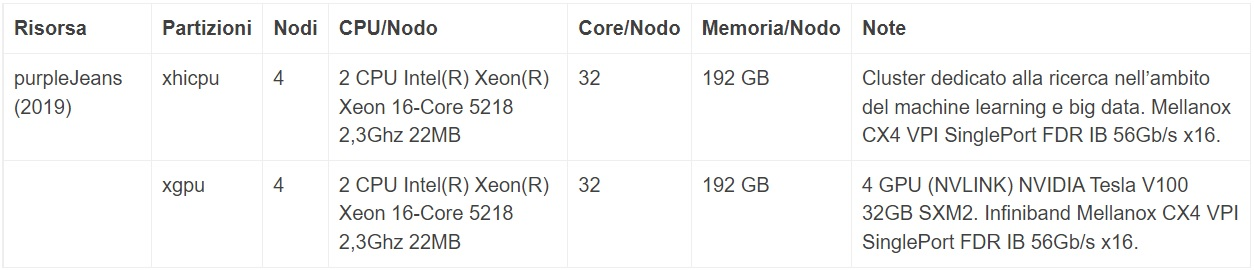
\includegraphics[scale=0.5]{images/chapter2/purple_jeans.jpg}
    \caption[Scheda tecnica di purpleJeans.]{Scheda tecnica di purpleJeans. \\
    Fonte: \url{https://rcf.uniparthenope.it/it/userguide/}}
    \label{fig:purple_jeans}
\end{figure}


L'utilizzo di purpleJeans è stato fondamentale nell'ottenimento dei risultati del docking proposti per il software AutoDock Vina.

\subsection{Google Colab}
Nonostante esistano diversi servizi di cloud computing, Google Colab è una piattaforma Cloud che permette di eseguire codice direttamente dal browser, sfruttando la potenza di calcolo messa a disposizione da Google ed attraverso i Jupyter Notebook, documenti interattivi in cui è possibile alternare paragrafi testuali a blocchi di codice eseguibili, scritti in Python oppure Shell scripting. 
L'utilizzo di Google Colab ha permesso l'ottenimento dei risultati relativi al docking con GNINA, sfruttando il tipo di runtime GPU, in maniera gratuita seppur con qualche limitazione sulla durata di utilizzo del servizio. 
